% Options for packages loaded elsewhere
\PassOptionsToPackage{unicode}{hyperref}
\PassOptionsToPackage{hyphens}{url}
%
\documentclass[
]{article}
\usepackage{amsmath,amssymb}
\usepackage{lmodern}
\usepackage{iftex}
\ifPDFTeX
  \usepackage[T1]{fontenc}
  \usepackage[utf8]{inputenc}
  \usepackage{textcomp} % provide euro and other symbols
\else % if luatex or xetex
  \usepackage{unicode-math}
  \defaultfontfeatures{Scale=MatchLowercase}
  \defaultfontfeatures[\rmfamily]{Ligatures=TeX,Scale=1}
\fi
% Use upquote if available, for straight quotes in verbatim environments
\IfFileExists{upquote.sty}{\usepackage{upquote}}{}
\IfFileExists{microtype.sty}{% use microtype if available
  \usepackage[]{microtype}
  \UseMicrotypeSet[protrusion]{basicmath} % disable protrusion for tt fonts
}{}
\makeatletter
\@ifundefined{KOMAClassName}{% if non-KOMA class
  \IfFileExists{parskip.sty}{%
    \usepackage{parskip}
  }{% else
    \setlength{\parindent}{0pt}
    \setlength{\parskip}{6pt plus 2pt minus 1pt}}
}{% if KOMA class
  \KOMAoptions{parskip=half}}
\makeatother
\usepackage{xcolor}
\usepackage[margin=1in]{geometry}
\usepackage{color}
\usepackage{fancyvrb}
\newcommand{\VerbBar}{|}
\newcommand{\VERB}{\Verb[commandchars=\\\{\}]}
\DefineVerbatimEnvironment{Highlighting}{Verbatim}{commandchars=\\\{\}}
% Add ',fontsize=\small' for more characters per line
\usepackage{framed}
\definecolor{shadecolor}{RGB}{248,248,248}
\newenvironment{Shaded}{\begin{snugshade}}{\end{snugshade}}
\newcommand{\AlertTok}[1]{\textcolor[rgb]{0.94,0.16,0.16}{#1}}
\newcommand{\AnnotationTok}[1]{\textcolor[rgb]{0.56,0.35,0.01}{\textbf{\textit{#1}}}}
\newcommand{\AttributeTok}[1]{\textcolor[rgb]{0.77,0.63,0.00}{#1}}
\newcommand{\BaseNTok}[1]{\textcolor[rgb]{0.00,0.00,0.81}{#1}}
\newcommand{\BuiltInTok}[1]{#1}
\newcommand{\CharTok}[1]{\textcolor[rgb]{0.31,0.60,0.02}{#1}}
\newcommand{\CommentTok}[1]{\textcolor[rgb]{0.56,0.35,0.01}{\textit{#1}}}
\newcommand{\CommentVarTok}[1]{\textcolor[rgb]{0.56,0.35,0.01}{\textbf{\textit{#1}}}}
\newcommand{\ConstantTok}[1]{\textcolor[rgb]{0.00,0.00,0.00}{#1}}
\newcommand{\ControlFlowTok}[1]{\textcolor[rgb]{0.13,0.29,0.53}{\textbf{#1}}}
\newcommand{\DataTypeTok}[1]{\textcolor[rgb]{0.13,0.29,0.53}{#1}}
\newcommand{\DecValTok}[1]{\textcolor[rgb]{0.00,0.00,0.81}{#1}}
\newcommand{\DocumentationTok}[1]{\textcolor[rgb]{0.56,0.35,0.01}{\textbf{\textit{#1}}}}
\newcommand{\ErrorTok}[1]{\textcolor[rgb]{0.64,0.00,0.00}{\textbf{#1}}}
\newcommand{\ExtensionTok}[1]{#1}
\newcommand{\FloatTok}[1]{\textcolor[rgb]{0.00,0.00,0.81}{#1}}
\newcommand{\FunctionTok}[1]{\textcolor[rgb]{0.00,0.00,0.00}{#1}}
\newcommand{\ImportTok}[1]{#1}
\newcommand{\InformationTok}[1]{\textcolor[rgb]{0.56,0.35,0.01}{\textbf{\textit{#1}}}}
\newcommand{\KeywordTok}[1]{\textcolor[rgb]{0.13,0.29,0.53}{\textbf{#1}}}
\newcommand{\NormalTok}[1]{#1}
\newcommand{\OperatorTok}[1]{\textcolor[rgb]{0.81,0.36,0.00}{\textbf{#1}}}
\newcommand{\OtherTok}[1]{\textcolor[rgb]{0.56,0.35,0.01}{#1}}
\newcommand{\PreprocessorTok}[1]{\textcolor[rgb]{0.56,0.35,0.01}{\textit{#1}}}
\newcommand{\RegionMarkerTok}[1]{#1}
\newcommand{\SpecialCharTok}[1]{\textcolor[rgb]{0.00,0.00,0.00}{#1}}
\newcommand{\SpecialStringTok}[1]{\textcolor[rgb]{0.31,0.60,0.02}{#1}}
\newcommand{\StringTok}[1]{\textcolor[rgb]{0.31,0.60,0.02}{#1}}
\newcommand{\VariableTok}[1]{\textcolor[rgb]{0.00,0.00,0.00}{#1}}
\newcommand{\VerbatimStringTok}[1]{\textcolor[rgb]{0.31,0.60,0.02}{#1}}
\newcommand{\WarningTok}[1]{\textcolor[rgb]{0.56,0.35,0.01}{\textbf{\textit{#1}}}}
\usepackage{graphicx}
\makeatletter
\def\maxwidth{\ifdim\Gin@nat@width>\linewidth\linewidth\else\Gin@nat@width\fi}
\def\maxheight{\ifdim\Gin@nat@height>\textheight\textheight\else\Gin@nat@height\fi}
\makeatother
% Scale images if necessary, so that they will not overflow the page
% margins by default, and it is still possible to overwrite the defaults
% using explicit options in \includegraphics[width, height, ...]{}
\setkeys{Gin}{width=\maxwidth,height=\maxheight,keepaspectratio}
% Set default figure placement to htbp
\makeatletter
\def\fps@figure{htbp}
\makeatother
\setlength{\emergencystretch}{3em} % prevent overfull lines
\providecommand{\tightlist}{%
  \setlength{\itemsep}{0pt}\setlength{\parskip}{0pt}}
\setcounter{secnumdepth}{-\maxdimen} % remove section numbering
\ifLuaTeX
  \usepackage{selnolig}  % disable illegal ligatures
\fi
\IfFileExists{bookmark.sty}{\usepackage{bookmark}}{\usepackage{hyperref}}
\IfFileExists{xurl.sty}{\usepackage{xurl}}{} % add URL line breaks if available
\urlstyle{same} % disable monospaced font for URLs
\hypersetup{
  pdftitle={SCIENVI201 Ecology Spring 2022},
  hidelinks,
  pdfcreator={LaTeX via pandoc}}

\title{SCIENVI201EcologySpring2022}
\author{}
\date{\vspace{-2.5em}Last updated: 2023-01-23}

\begin{document}
\maketitle

{
\setcounter{tocdepth}{3}
\tableofcontents
}
\hfill\break

\hypertarget{introduction}{%
\section{Introduction}\label{introduction}}

This page collects workshop materials, data sources and supplementary
materials for the data-driven assignments in the Spring 2022 edition of
Ecology at UCR. You can also access the related files directly on
\href{https://github.com/ucrdatacenter/projects/tree/main/SCIENVI201/2022h1}{Github}.

If you have any questions related to the assignment do not hesitate to
reach Bianka during Data Center office hours (held every Wednesday 17:00
- 19:00 on
\href{https://universitycollegeroosevelt.zoom.us/j/2831128718?pwd=UmRuSzVqSTZyMndDbDRGSkV5VWFVQT09}{Zoom}).
There is no need to sign up in advance to join office hours. If this
time is inconvenient for you feel free to write Bianka an email
(\href{mailto:ucrdatacenter@ucr.nl}{\nolinkurl{ucrdatacenter@ucr.nl}})
to schedule an individual meeting.

\hfill\break

\hypertarget{working-with-r-and-rstudio}{%
\section{Working with R and RStudio}\label{working-with-r-and-rstudio}}

\hypertarget{recommended-reading}{%
\subsection{Recommended reading}\label{recommended-reading}}

It is highly recommended that you read the sections 2, 3.1-3.4 and 4-6
of
\href{https://github.com/ClaudiaBrauer/A-very-short-introduction-to-R/blob/master/documents/A\%20(very)\%20short\%20introduction\%20to\%20R.pdf}{A
(very) short introduction to R} and sections 1-4 of
\href{http://r-statistics.co/ggplot2-Tutorial-With-R.html\#6.1\%20Make\%20a\%20time\%20series\%20plot\%20(using\%20ggfortify)}{How
to make any plot in ggplot2?} before starting working with R.

\hypertarget{installing-r-and-rstudio}{%
\subsection{Installing R and RStudio}\label{installing-r-and-rstudio}}

R is the programming language that you use when working with data.
RStudio is a development environment that makes working with R much more
convenient. Both are free to download and install.

To download R, go to
\href{https://cloud.r-project.org/}{cloud.r-project.org} and follow the
instructions on the page. To download RStudio, go to
\href{https://www.rstudio.com/products/rstudio/download/}{rstudio.com/products/rstudio/download},
scroll down and download the file recommended for your operating system.

When installing, you can always stick to the default settings, unless
you have different preferences.

In case you get stuck at any point, or would like more guidance in the
installation process, feel free to check out any of the following links:

\begin{itemize}
\tightlist
\item
  \href{https://www.dataquest.io/blog/tutorial-getting-started-with-r-and-rstudio/}{Tutorial:
  Getting Started with R and RStudio}
\item
  \href{https://www.youtube.com/watch?v=0Qu7Jg1Jw5A}{R Tutorial: How to
  install R and R studio (video)}
\end{itemize}

\hypertarget{creating-a-project-in-rstudio}{%
\subsection{Creating a project in
RStudio}\label{creating-a-project-in-rstudio}}

It is convenient to create an R project for an assignment that you are
working on. A project is basically a folder that stores all files
related to the assignment.

You can create a project as follows:

\begin{itemize}
\tightlist
\item
  Open RStudio and click on ``Project: (None)'' in the top right corner.
\item
  Open the dropdown window and click on ``New Project\ldots.''
\item
  In the popup window select ``New Directory'', then ``New Project.''
\item
  Choose a sensible name for your project and enter it as the Directory
  Name. You can either use the default file path or change it by
  clicking ``Browse\ldots{}'' next to ``Create project as a subdirectory
  of:.''
\item
  Finally, click on ``Create project.''
\end{itemize}

After a project is created, there are two easy ways of accessing it. You
can either use the same dropdown window in the top right corner of
RStudio that you used to create the project, and click on the name of
the project there, or you can find the project folder within your files
and click on the file with the .Rproj extension.

\hfill\break

\hypertarget{assignment}{%
\section{Assignment}\label{assignment}}

\hypertarget{nitrogen-deposition-effect-on-biodiversity}{%
\section*{\texorpdfstring{\textbf{Nitrogen deposition effect on
biodiversity}}{Nitrogen deposition effect on biodiversity}}\label{nitrogen-deposition-effect-on-biodiversity}}

\includegraphics{https://user-images.githubusercontent.com/84587448/144092109-7298977c-a6af-4146-9dde-54d51b3741b4.jpg}

Nitrogen deposition is one of the main causes of current biodiversity
decline (Payne, et a., 2013). This is mainly due to highly intensified
agricultural practices which are very common, here, in the Netherlands.
Therefore, environmentalists and ecologists have had numerous debates in
recent years on how to analyze and tackle this biodiversity decline due
to nitrogen. What is the response of individual species to increasing
Nitrogen levels? Which species are negatively impacted and might some
even benefit form this environmental change? As an ecologist, you need
to know what is the species distribution and how does it correlate with
increasing nitrogen deposition levels to be able to draw the right
conclusion and to suggest appropriate action plans for species
protection. In this assignment you will work with external source of
species occurrences, will correlate these to nitrogen deposition in the
Netherlands, and perform a statistical test to see what relationship
there is between nitrogen deposition and the occurrences of a chosen
species.

\hypertarget{data}{%
\subsection{DATA}\label{data}}

Data on organism occurrences can be directly downloaded in a csv file
from \href{https://www.gbif.org/}{gbif.org}.\\
Data on nitrogen deposition levels in the Netherlands can be downloaded
from RIVM website:
\href{https://www.rivm.nl/gcn-gdn-kaarten/depositiekaarten/cijfers-achter-depositiekaarten/gdn-depositiebestanden-achterliggende-jaren}{rivm.nl}.

\hypertarget{learning-outcomes}{%
\subsection{LEARNING OUTCOMES}\label{learning-outcomes}}

While completing this assignment, a student can gain practice in
performing research with data from an external source as well as develop
multiple R skills such as:

\begin{itemize}
\tightlist
\item
  obtaining and importing data from an online source to R,
\item
  filtering and adjusting data to reach a set of desired information
  only,
\item
  visualizing species occurrences and Nitrogen deposition levels,
\item
  visualizing graphs in R,
\item
  performing statistical test.
\end{itemize}

\hypertarget{research-focus}{%
\subsection{RESEARCH FOCUS}\label{research-focus}}

What is the relationship between species occurrences and nitrogen
deposition levels?

\hypertarget{literature}{%
\subsection{LITERATURE}\label{literature}}

Suggested literature for further information:\\

\emph{de Vries, W., Erisman, J. W., Spranger, T., Stevens, C. J., \& van
den Berg, L. (2011). Nitrogen as a threat to European terrestrial
biodiversity. The European nitrogen assessment: sources, effects and
policy perspectives, 436-494.}

\emph{Payne, R. J., Dise, N. B., Stevens, C. J., \& Gowing, D. J.
(2013). Impact of nitrogen deposition at the species level. Proceedings
of the National Academy of Sciences, 110(3), 984-987.}

\emph{Stevens, C. J., David, T. I., \& Storkey, J. (2018). Atmospheric
nitrogen deposition in terrestrial ecosystems: Its impact on plant
communities and consequences across trophic levels. Functional ecology,
32(7), 1757-1769.}

\hfill\break

\hypertarget{instructions}{%
\section{Instructions}\label{instructions}}

These assignment instructions serve you as a guide in completing your
original assignment. Here, I will walk you step by step through an
example of the assignment. Once you complete this, you can start with
your own variation of the assignment. Creativity is very welcome. In
your version of the assignment you choose:

\begin{itemize}
\tightlist
\item
  species of an interest
\item
  year (of Nitrogen deposition and species ocurrences).
\end{itemize}

\hypertarget{the-correlation-between-chaffinch-fringilla-coelebs-and-nitrogen-deposition-levels-in-the-netherlands}{%
\section*{\texorpdfstring{\textbf{The correlation between Chaffinch,
\emph{Fringilla coelebs}, and Nitrogen deposition levels in the
Netherlands}}{The correlation between Chaffinch, Fringilla coelebs, and Nitrogen deposition levels in the Netherlands}}\label{the-correlation-between-chaffinch-fringilla-coelebs-and-nitrogen-deposition-levels-in-the-netherlands}}

\includegraphics{https://user-images.githubusercontent.com/84587448/148916498-2fb3d7c6-5d03-4c85-9a0f-68f5efff1efe.jpg}

\hfill\break

At this step it is assumed that you have:

\begin{itemize}
\tightlist
\item
  installed R and RStudio (the working environment for R language),
\item
  created an R project for this assignment,
\item
  read the recommended reading.
\end{itemize}

Now, open the R project you have created according to the instructions
above. RStudio interface consists of four windows. Top right is the
environment window storing the data and values currently in R memory.
Bottom right is the plots, packages, and help window. Bottom left is the
console window where you can type commands which R will execute without
saving them. Top left is the script window which holds collections of
commands which can be edited and saved. In this assignment we will write
our code in the top left window, R Script file. If you cannot see this
window click File on the top left -\textgreater{} New File
-\textgreater{} R Script.\\
Two notes before we dive into the assignment: * if you have troubles
understanding a code, the easiest way how to learn more about it is
typing \emph{?codename} into the console and pressing enter. For example
\emph{?library()} or \emph{?ggplot()}. * to run a code in console
(bottom left window) you press Enter, to run a code in script (top left
window) you press Ctrl + Enter

\hypertarget{libraries}{%
\subsection{LIBRARIES}\label{libraries}}

An R library or an R package is a collection of functions, data, and
documentation that allows you for a clean workflow. To be able to access
a package you first need to install it with the code
\emph{install.packages(\ldots)}. You only need to install a package
once. However, in order to be able to work with the packages in your
RStudio environment you need to load them with the code
\emph{library(\ldots)}. It is a good practice to have your libraries
loaded on the top of your R Script so you can always come back to your
code knowing which libraries you used.

In this assignment we will be using the following packages.

\begin{Shaded}
\begin{Highlighting}[]
\FunctionTok{install.packages}\NormalTok{(}\StringTok{"tidyverse"}\NormalTok{)}
\FunctionTok{install.packages}\NormalTok{(}\StringTok{"tabularaster"}\NormalTok{)}
\FunctionTok{install.packages}\NormalTok{(}\StringTok{"terra"}\NormalTok{)}
\FunctionTok{install.packages}\NormalTok{(}\StringTok{"sf"}\NormalTok{)}
\FunctionTok{install.packages}\NormalTok{(}\StringTok{"readr"}\NormalTok{)}
\FunctionTok{install.packages}\NormalTok{(}\StringTok{"tidymodels"}\NormalTok{)}
\end{Highlighting}
\end{Shaded}

The next step is to load the libraries in your RStudio, so they are
ready to be used. To keep an overview, every section has a comment which
says which library you are using.

\begin{Shaded}
\begin{Highlighting}[]
\FunctionTok{library}\NormalTok{(tabularaster)}
\FunctionTok{library}\NormalTok{(terra)}
\FunctionTok{library}\NormalTok{(sf)}
\FunctionTok{library}\NormalTok{(readr)}
\FunctionTok{library}\NormalTok{(tidymodels)}
\FunctionTok{library}\NormalTok{(tidyverse)}
\end{Highlighting}
\end{Shaded}

\hypertarget{data-import}{%
\subsection{DATA IMPORT}\label{data-import}}

\hypertarget{nitrogen-data}{%
\paragraph{Nitrogen data}\label{nitrogen-data}}

Go to the website:
\href{https://www.rivm.nl/gcn-gdn-kaarten/depositiekaarten/cijfers-achter-depositiekaarten/gdn-depositiebestanden-achterliggende-jaren}{rivm.nl},
and download \textbf{total Nitrogen deposition (Total stikstof (N))}
from the year 2018 (ndep 2018). Once downloaded, you can see that the
data is in a zipped file which cannot be worked with in RStudio.
Therefore, \emph{extract all} with the right click, and save the
extracted data into a new created file called Data in your Project
folder. I renamed the file from depo\_ntot\_2018 to nitrogen for a
simple overview, but you can order your files according to your own
preferences. However, remember to update your code according to your
files' names. Now, we can import the data on nitrogen deposition levels
to our RStudio. We will do so with the code \emph{rast(\ldots)} which
imports data from a raster file. Raster file stores image data in a
matrix of cells organized in rows and columns. Next, we want to call
this imported data Nitrogen\_2018. We do so with the symbol \textless-.
If the importing was successful we should see Nitrogen\_2018 data in our
global environment (top right window).

\begin{Shaded}
\begin{Highlighting}[]
\CommentTok{\# library used: library(terra)}
\NormalTok{Nitrogen\_2018 }\OtherTok{\textless{}{-}} 
  \FunctionTok{rast}\NormalTok{(}\StringTok{"https://raw.githubusercontent.com/ucrdatacenter/projects/main/SCIENVI201/2022h1/Data/nitrogen/depo\_ntot\_2018.asc"}\NormalTok{)}
\end{Highlighting}
\end{Shaded}

Let's see how does the Nitrogen deposition map looks like. At first, we
want to let R know which data do we want to work with by typing down its
name, Nitrogen\_2018. Now, looking at the code, we can see that we
connect multiple functions with this magical \%\textgreater\% sign. This
symbol \%\textgreater\% is called a pipe. A pipe allows us to connect
multiple operations in a simple format so it is easy to understand and
read. If you are interested in reading more about pipes, you can do so
\href{https://r4ds.had.co.nz/pipes.html}{here}. Next, we rewrite the
Nitrogen\_2018 data into a data frame, table structure of data.
Followingly, we rewrite it into a tibble, a simple version of data frame
which only shows first 10 rows of a data set. Run the code and look at
the result, a tibble, in the console. Our tibble consists of three
variables:

\begin{itemize}
\tightlist
\item
  x variable (longitude),
\item
  y variable (latitude),
\item
  depo\_ntot\_2018 variable (the level of deposition in mol/(ha.yea)).
\end{itemize}

\begin{Shaded}
\begin{Highlighting}[]
\CommentTok{\# library used: library(tidyverse)}
\NormalTok{Nitrogen\_2018 }\SpecialCharTok{\%\textgreater{}\%} 
  \FunctionTok{as.data.frame}\NormalTok{(}\AttributeTok{xy =}\NormalTok{ T) }\SpecialCharTok{\%\textgreater{}\%} 
  \FunctionTok{as\_tibble}\NormalTok{() }
\end{Highlighting}
\end{Shaded}

\begin{verbatim}
## # A tibble: 43,959 x 3
##         x      y depo_ntot_2018
##     <dbl>  <dbl>          <dbl>
##  1 236500 621500           602.
##  2 237500 621500           605.
##  3 238500 621500           608.
##  4 213500 620500           537 
##  5 214500 620500           542.
##  6 215500 620500           546.
##  7 216500 620500           550.
##  8 217500 620500           551.
##  9 218500 620500           555.
## 10 219500 620500           556.
## # ... with 43,949 more rows
\end{verbatim}

Having understood the structure of our data, we move forward with
visualizing it. To previous lines of code we attach a ggplot. As you
have read in your recommended reading, ggplot is a graphical framework
for R. Our data set is already known and therefore we do not need to
specify it anymore in the ggplot() line of code as a data argument.
However, we still need to specify the aesthetic mapping, the x and y
coordinates of our graph. In our case, it is simple as our variables are
called x (longitude) and y (latitude). Our third aesthetic is a fill
argument which enables us to visualize a third variable. In our case,
the level of nitrogen. Once the variables are defined, we choose how do
we want to visualize them. Since our data is in a raster format we will
use geom\_raster().

\begin{Shaded}
\begin{Highlighting}[]
\CommentTok{\# library used: library(tidyverse)}
\NormalTok{Nitrogen\_2018 }\SpecialCharTok{\%\textgreater{}\%} 
  \FunctionTok{as.data.frame}\NormalTok{(}\AttributeTok{xy =}\NormalTok{ T) }\SpecialCharTok{\%\textgreater{}\%} 
  \FunctionTok{as\_tibble}\NormalTok{() }\SpecialCharTok{\%\textgreater{}\%} 
  \FunctionTok{ggplot}\NormalTok{(}\FunctionTok{aes}\NormalTok{(}\AttributeTok{x =}\NormalTok{ x, }\AttributeTok{y =}\NormalTok{ y, }\AttributeTok{fill =}\NormalTok{ depo\_ntot\_2018)) }\SpecialCharTok{+} 
  \FunctionTok{geom\_raster}\NormalTok{()}
\end{Highlighting}
\end{Shaded}

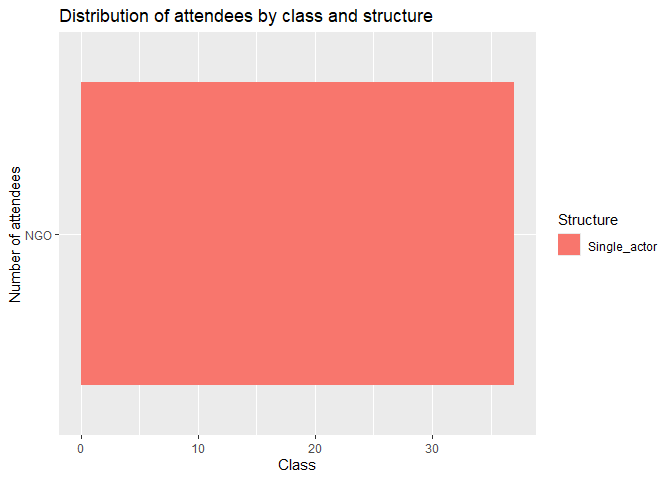
\includegraphics{SCIENVI201_2022h1_files/figure-latex/unnamed-chunk-5-1.pdf}

\hypertarget{species-data}{%
\paragraph{Species data}\label{species-data}}

Go to the website: \href{https://www.gbif.org/}{gbif.org}, click get
data (toolbar on the top) and select occurrences. Now select, the
occurrences of your species in your preferred region. Go to the toolbar
on the left, under Scientific name type: \textbf{Fringilla coelebs}, in
Year select: \textbf{2018}, and finally in Country or area select:
\textbf{Netherlands}. Click DOWNLOAD, create an account, and select
SIMPLE in download options. This step might take a little while, as the
request needs to be processed. In the meanwhile, create a chaffinch
folder in your Data folder where you will store all the information on
your species. Once the file is ready, click download, and save the data.
It is again a zipped file which needs to be extracted. With the right
click select \emph{extract all} and save the data into chaffinch file in
the Data folder. As a last step, rename the extracted csv file to
chaffinch\_2018. Now, we can import the data on chaffinch,
\emph{Fringilla coelebs}, to our Rstudio. There are two ways how to do
this. One of them is selecting Files in your bottom right window in
RStudio -\textgreater{} Data -\textgreater{} chaffinch\_2018
-\textgreater{} Import Dataset\ldots{} -\textgreater{} selecting Tab in
the Delimeter options in the bottom toolbar -\textgreater{} import.
Second option how to import the data is by using the code
\emph{read\_delim(``pathway'', delim = ``\t", escape\_double = FALSE,
trm\_ws = TRUE)} as indicated below. The argument delim defines how is
the data separated. In our case it is a tab (\textbackslash t).
Similarly to how we named the nitrogen data, we now call our species
occurrences data Chaffinch\_2018 with the symbol \textless-.

\begin{Shaded}
\begin{Highlighting}[]
\CommentTok{\# library used: library(readr)}
\NormalTok{Chaffinch\_2018 }\OtherTok{\textless{}{-}} 
  \FunctionTok{read\_delim}\NormalTok{(}\StringTok{"https://raw.githubusercontent.com/ucrdatacenter/projects/main/SCIENVI201/2022h1/Data/chaffinch/chaffinch\_2018.csv"}\NormalTok{,}
             \AttributeTok{delim =} \StringTok{"}\SpecialCharTok{\textbackslash{}t}\StringTok{"}\NormalTok{, }\AttributeTok{escape\_double =} \ConstantTok{FALSE}\NormalTok{, }\AttributeTok{trim\_ws =} \ConstantTok{TRUE}\NormalTok{)}
\end{Highlighting}
\end{Shaded}

Let's view the data set on chaffinch. This can be simply done either by
clicking on Chaffinch\_2018 in the global environment or by using code
\emph{view()}.

\begin{Shaded}
\begin{Highlighting}[]
\NormalTok{Chaffinch\_2018 }\SpecialCharTok{\%\textgreater{}\%} \FunctionTok{view}\NormalTok{()}
\end{Highlighting}
\end{Shaded}

Looking at the data set, we can see that it is quiet extensive having 50
columns and over 60000 observations (rows). We can also notice how are
coordinate variables (longitude and latitude) called as we will need it
in the next step. Now, we will visualize our species occurrences on a
map so we have an idea of their distribution. This time, we need to
specify the data we want to visualize in ggplot() as data = \ldots{}
argument. We want to see occurrences points on a coordinate map, in
other words, dots on a graph. Therefore, we will choose geom\_point() as
a layer how to visualize our plot. Our mapping aesthetics are for x
coordinate longitude (decimalLongitude) and for y coordinate latitude
(decimalLatitude).

\begin{Shaded}
\begin{Highlighting}[]
\CommentTok{\# library used: library(tidyverse)}
\FunctionTok{ggplot}\NormalTok{(}\AttributeTok{data =}\NormalTok{ Chaffinch\_2018) }\SpecialCharTok{+}
  \FunctionTok{geom\_point}\NormalTok{(}\FunctionTok{aes}\NormalTok{(}\AttributeTok{x =}\NormalTok{ decimalLongitude, }\AttributeTok{y =}\NormalTok{ decimalLatitude))}
\end{Highlighting}
\end{Shaded}

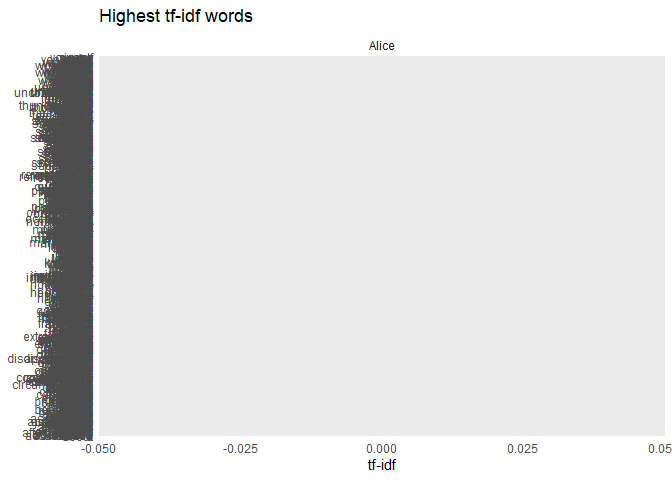
\includegraphics{SCIENVI201_2022h1_files/figure-latex/unnamed-chunk-8-1.pdf}

We could have seen that the data set is quiet big. However, we do not
need all the information. Therefore, in the next step we will clean our
data set to our preferred size.

\hypertarget{data-tidying}{%
\subsection{DATA TIDYING}\label{data-tidying}}

For the following part of the assignment please read Introduction to
\href{https://wec.wur.nl/r/spatial/introduction.html}{Spatial Data and
Analysis in R}, sections 1.1 and 1.2.

In this following code we select the variables with which we will be
working: species names (species), longitude (decimalLongitude), and
latitude (decimalLatitude) with the code \emph{select()}. Furthermore,
we omit all the unknown variables to avoid errors later on with the code
\emph{na.omit()}. As a last step, we convert our data frame
Chaffinch\_2018 into an sf object. This simply means that our spatial
coordinate variables, the latitude and longitude, will be merged from
two variables into one variable.

\begin{Shaded}
\begin{Highlighting}[]
\CommentTok{\# library used: library(tidyverse) and library(sf)}
\NormalTok{Chaffinch\_2018 }\OtherTok{\textless{}{-}}\NormalTok{ Chaffinch\_2018 }\SpecialCharTok{\%\textgreater{}\%}
\NormalTok{  dplyr}\SpecialCharTok{::}\FunctionTok{select}\NormalTok{(species, decimalLongitude, decimalLatitude) }\SpecialCharTok{\%\textgreater{}\%} \CommentTok{\# in this case you can notice that we wrote down dplyr::select instead of just typing command select(). This is because the command select() is in two of our libraries. Therefore, we wanted to specify that this select is from dplyr package which is within tidyverse.}
  \FunctionTok{na.omit}\NormalTok{() }\SpecialCharTok{\%\textgreater{}\%}
  \FunctionTok{st\_as\_sf}\NormalTok{(}\AttributeTok{coords =} \FunctionTok{c}\NormalTok{(}\StringTok{"decimalLongitude"}\NormalTok{,}\StringTok{"decimalLatitude"}\NormalTok{)) }
\end{Highlighting}
\end{Shaded}

When working with geo-spatial data, we can come across various versions
of coordinate systems. Therefore, our next step is to check whether our
two geo-spatial data (Nitrogen and Chaffinch) is in the same coordinate
system. The code \emph{crs(data)} tells us in which coordinate system
the geo-spatial data is. Here, the Nitrogen deposition file does not
have it defined, but reading the information on the data set we know
that the data set is in Amersfoort coordinate system. Therefore, we can
tell the Nitrogen\_2018 that it is in this format. Similarly, all data
occurrences from global biodiversity information facility (gbif) are
recorded in gobal geographic coordinate system WGS84 (EPSG:4326).
Therefore, we can also set the coordinate system for Chaffinch\_2018.

\begin{Shaded}
\begin{Highlighting}[]
\CommentTok{\# libraries used: library(sf) and library(terra)}
\FunctionTok{crs}\NormalTok{(Nitrogen\_2018) }\OtherTok{\textless{}{-}} \StringTok{"+init=epsg:28992"}
\FunctionTok{st\_crs}\NormalTok{(Chaffinch\_2018) }\OtherTok{\textless{}{-}} \StringTok{"+init=epsg:4326"}
\end{Highlighting}
\end{Shaded}

Next we can transform the chaffinch coordinate system into the same
coordinate system as Nitrogen\_2018 with the code
\emph{st\_transform()}.

\begin{Shaded}
\begin{Highlighting}[]
\NormalTok{Chaffinch\_2018 }\OtherTok{\textless{}{-}} \FunctionTok{st\_transform}\NormalTok{(Chaffinch\_2018, }\DecValTok{28992}\NormalTok{)}
\end{Highlighting}
\end{Shaded}

Now, we do not only want to be able to see our data on a graph but also
in a numeric data set. In another words, we want to see which
geo-spatial point belongs to which Nitrogen level and species occurring.
Therefore, we want to merge these two files (Nitrogen\_2018 and
Chaffinch\_2018) and write it into a table complete\_data. We can do
this with the code \emph{extract()}. How does that work? Imagine having
two paper maps laying on top of each other on a table. Now, you take a
pin and you pin it across both of the papers from top down. R takes the
information from both of the maps on this exact place where the pin was
pinned and stores it in a row. Once extracted, you store this
information in a tibble with \emph{as\_tibble()}. In the next step we
want to add a species variable to the complete\_data table which can be
done with the code \emph{mutate()}. This will help us in visualization
in the next step.

\begin{Shaded}
\begin{Highlighting}[]
\CommentTok{\#library used: library(terra)}

\NormalTok{complete\_data }\OtherTok{\textless{}{-}}\NormalTok{ terra}\SpecialCharTok{::}\FunctionTok{extract}\NormalTok{(Nitrogen\_2018, }\FunctionTok{vect}\NormalTok{(Chaffinch\_2018), }\AttributeTok{cells =}\NormalTok{ T, }\AttributeTok{xy =}\NormalTok{ T) }\SpecialCharTok{\%\textgreater{}\%} \FunctionTok{as\_tibble}\NormalTok{() }

\NormalTok{complete\_data }\OtherTok{\textless{}{-}}\NormalTok{ complete\_data }\SpecialCharTok{\%\textgreater{}\%} 
  \FunctionTok{mutate}\NormalTok{(}\AttributeTok{species =} \StringTok{"Fringilla coelebs"}\NormalTok{)}
\end{Highlighting}
\end{Shaded}

\hypertarget{plotting}{%
\subsection{PLOTTING}\label{plotting}}

Once, we have our data sets in our desired format, we would like to look
at a graph which would show us whether there is some relationship
between the level of Nitrogen and species occurrences. In the following
lines of code, we have three various graphs. You need to justify
yourself which one is the most informative. While building the graphs
think of your dependent and independent variables. Which one of the two
variable should be on the x axis and which one should be on the y axis?
Why?

From your statistics class you might remember that a boxplot shows the
distribution of a numeric data and its skewness across quartiles with
middle line displaying the median. In R, we can simply built boxplot
with the ggplot. We need to specify the data, the x variable, and the y
variable. The labs() code enables us to add additional description to
our graph such as: name of axes, title, caption, etc..

\begin{Shaded}
\begin{Highlighting}[]
\CommentTok{\# library used: library(tidyverse)}
\CommentTok{\# BOXPLOT}
\FunctionTok{ggplot}\NormalTok{(}\AttributeTok{data =}\NormalTok{ complete\_data) }\SpecialCharTok{+} 
  \FunctionTok{geom\_boxplot}\NormalTok{(}\FunctionTok{aes}\NormalTok{(}\AttributeTok{x =}\NormalTok{ species, }\AttributeTok{y =}\NormalTok{ depo\_ntot\_2018)) }\SpecialCharTok{+}
  \FunctionTok{labs}\NormalTok{(}\AttributeTok{x =} \StringTok{"Chaffinch, Fringilla coelebs (n)"}\NormalTok{,}
      \AttributeTok{y =} \StringTok{"Nitrogen deposition (mol/(ha.year))"}\NormalTok{)}
\end{Highlighting}
\end{Shaded}

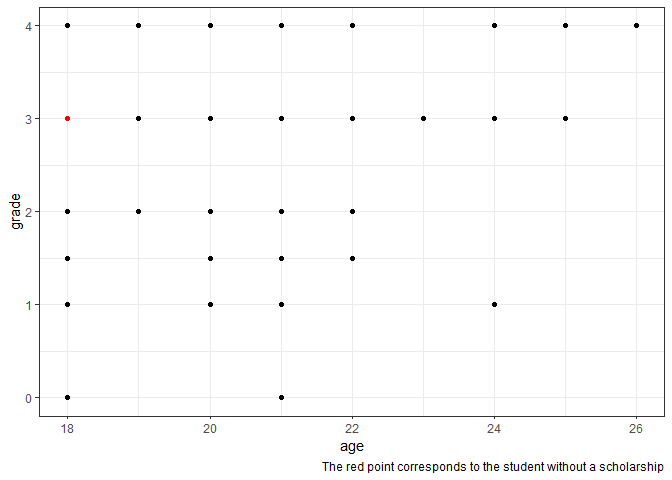
\includegraphics{SCIENVI201_2022h1_files/figure-latex/unnamed-chunk-13-1.pdf}

Our next type of graph is a histogram. A histogram displays data
distribution using rectangular bars. Just as we did with the boxplot, we
need to specify the data, x and y variables using ggplot(). You might
notice, that in the geom\_histogram code we added an extra argument
binwidth = \ldots{} . Binwidth groups observations that are very closely
related together. Therefore, it is easier for us to see the general
relationship. I believe that one picture sometimes shows more than a
thousand words. Therefore, to understand what binwidth does, try to set
binwidth to 1, run the code, and then set it to 100 (be sure to notice
the species frequency on y axis) and run it again. When binwidth is set
to 1, we see a lots of little correlations, but it is hard to observe
the general relationship.

\begin{Shaded}
\begin{Highlighting}[]
\CommentTok{\# library used: library(tidyverse)}
\CommentTok{\# HISTOGRAM}
\FunctionTok{ggplot}\NormalTok{(}\AttributeTok{data =}\NormalTok{ complete\_data) }\SpecialCharTok{+}
  \FunctionTok{geom\_histogram}\NormalTok{(}\FunctionTok{aes}\NormalTok{(}\AttributeTok{x =}\NormalTok{ depo\_ntot\_2018), }\AttributeTok{binwidth =} \DecValTok{100}\NormalTok{) }\SpecialCharTok{+}
  \FunctionTok{labs}\NormalTok{(}\AttributeTok{x =} \StringTok{"Nitrogen deposition (mol/(ha.year))"}\NormalTok{,}
      \AttributeTok{y =} \StringTok{"Chaffinch, Fringilla coelebs (n)"}\NormalTok{)}
\end{Highlighting}
\end{Shaded}

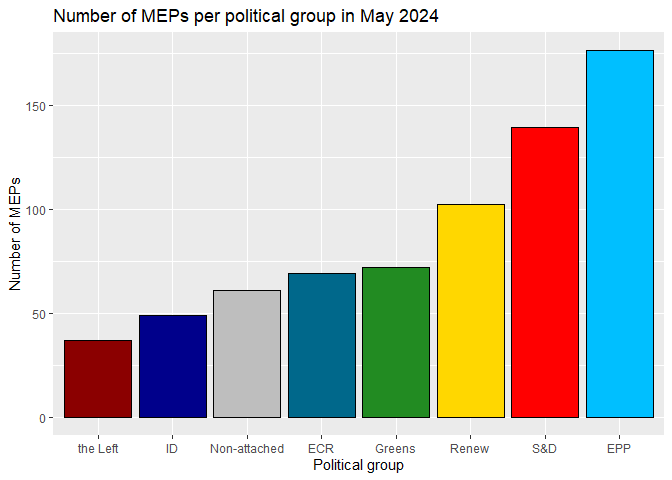
\includegraphics{SCIENVI201_2022h1_files/figure-latex/unnamed-chunk-14-1.pdf}

Lastly, we have a frequency polygon. Frequency polygon works similarly
to a histogram with the exception that it uses a line instead of bars
for the distribution display. The code is built in the very same way as
the code for the histogram visualization. The only difference is the
geom type.

\begin{Shaded}
\begin{Highlighting}[]
\CommentTok{\# library  used: library(tidyverse)}
\CommentTok{\# FREQUENCY POLYGON}
\FunctionTok{ggplot}\NormalTok{(}\AttributeTok{data =}\NormalTok{ complete\_data) }\SpecialCharTok{+}
  \FunctionTok{geom\_freqpoly}\NormalTok{(}\FunctionTok{aes}\NormalTok{(}\AttributeTok{x =}\NormalTok{ depo\_ntot\_2018), }\AttributeTok{binwidth =} \DecValTok{100}\NormalTok{) }\SpecialCharTok{+}
  \FunctionTok{labs}\NormalTok{(}\AttributeTok{title =} \StringTok{"Species occurences per Nitrogen deposition"}\NormalTok{,}
       \AttributeTok{x =} \StringTok{"Nitrogen deposition (mol/(ha.year))"}\NormalTok{,}
       \AttributeTok{y =} \StringTok{"Chaffinch (Fringilla coelebs) (n)"}\NormalTok{)}
\end{Highlighting}
\end{Shaded}

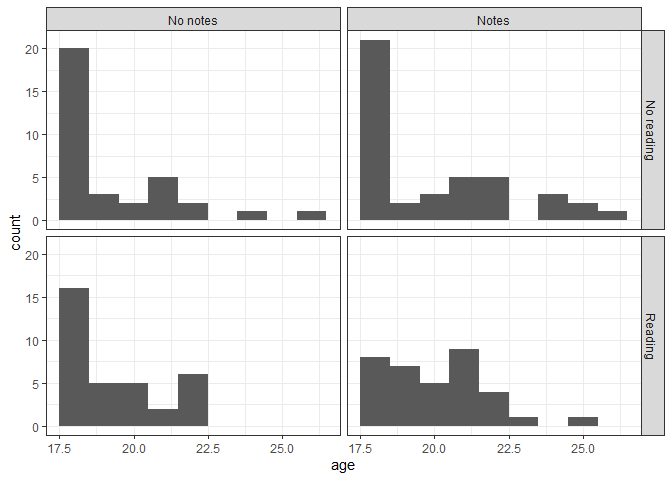
\includegraphics{SCIENVI201_2022h1_files/figure-latex/unnamed-chunk-15-1.pdf}

\hypertarget{statistical-analysis}{%
\subsection{STATISTICAL ANALYSIS}\label{statistical-analysis}}

After visually observing the relationship, we want to see the
quantitative analysis. First, we would like to adjust our data set. As
you might have noticed, in our complete\_data data frame, there is
always only one observation of a species per row. This means that we do
not know how many birds there are at a specific level of nitrogen.
However, we can do so with a few lines of code. We want to create a new
variable with the code \emph{mutate()} called bins. Just as we did in
the histogram and the frequency polygon, we want to group similar values
of observations together. In other words, we want to round them up to
100. Therefore we want our new variable, bins, to have rounded up values
of nitrogen deposition to 100. In the next step, we want to see how many
species are observed at the same level of nitrogen. Since there is
always just one species per row, we simply want to count the number of
rows with the same nitrogen value. Lastly, we want to rename the
variables according to our x and y axes, and omit the unknown variables
with the \emph{na.omit()}.

\begin{Shaded}
\begin{Highlighting}[]
\CommentTok{\# library used: library(tidyverse)}
\CommentTok{\# writing a table t with x (nitrogen levels) and y (species frequency) variables}
\NormalTok{t }\OtherTok{\textless{}{-}}\NormalTok{ complete\_data }\SpecialCharTok{\%\textgreater{}\%} 
  \FunctionTok{mutate}\NormalTok{(}\AttributeTok{bins =} \FunctionTok{round}\NormalTok{(depo\_ntot\_2018, }\AttributeTok{digits =} \SpecialCharTok{{-}}\DecValTok{2}\NormalTok{)) }\SpecialCharTok{\%\textgreater{}\%} 
  \FunctionTok{group\_by}\NormalTok{(bins) }\SpecialCharTok{\%\textgreater{}\%} 
  \FunctionTok{count}\NormalTok{() }\SpecialCharTok{\%\textgreater{}\%} 
  \FunctionTok{rename}\NormalTok{(}\AttributeTok{x =}\NormalTok{ bins,}
         \AttributeTok{y =}\NormalTok{ n) }\SpecialCharTok{\%\textgreater{}\%} 
  \FunctionTok{na.omit}\NormalTok{()}
\end{Highlighting}
\end{Shaded}

Now we want to visualize our newly made table t as a simple scatter plot
using \emph{geom\_point()}. On the top of that we would like to add a
parabola layer to see whether our data distribution could be quadratic.

\begin{Shaded}
\begin{Highlighting}[]
\CommentTok{\# visualizing the relationship}
\FunctionTok{ggplot}\NormalTok{(}\AttributeTok{data =}\NormalTok{ t, }\FunctionTok{aes}\NormalTok{(}\AttributeTok{x =}\NormalTok{ x, }\AttributeTok{y =}\NormalTok{ y, }\AttributeTok{group =} \DecValTok{1}\NormalTok{)) }\SpecialCharTok{+}
  \FunctionTok{geom\_point}\NormalTok{() }\SpecialCharTok{+}
  \FunctionTok{geom\_smooth}\NormalTok{(}\AttributeTok{method =} \StringTok{"lm"}\NormalTok{, }\AttributeTok{formula =}\NormalTok{ y }\SpecialCharTok{\textasciitilde{}} \FunctionTok{poly}\NormalTok{(x, }\DecValTok{2}\NormalTok{), }\AttributeTok{se =} \ConstantTok{FALSE}\NormalTok{) }\SpecialCharTok{+}
  \FunctionTok{labs}\NormalTok{(}\AttributeTok{title =} \StringTok{"Species occurences per Nitrogen deposition"}\NormalTok{,}
       \AttributeTok{x =} \StringTok{"Nitrogen deposition (mol/(ha.year))"}\NormalTok{,}
       \AttributeTok{y =} \StringTok{"Chaffinch (Fringilla coelebs) (n)"}\NormalTok{)}
\end{Highlighting}
\end{Shaded}

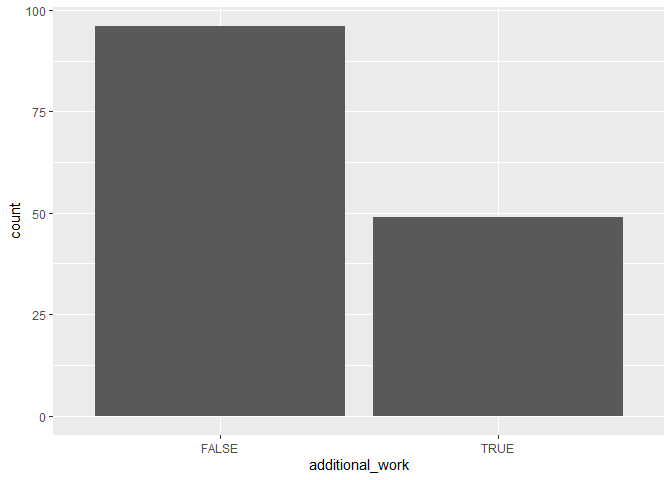
\includegraphics{SCIENVI201_2022h1_files/figure-latex/unnamed-chunk-17-1.pdf}

Our last step is to demonstrate results quantitatively. This can be done
with a linear model using code \emph{lm()}. Do not stress out now. The
aim of this assignment is not to learn linear modeling, but to get in
touch with basic skills in R and apply it to ecology. All you need to
know is that lm(y \textasciitilde{} poly(x, 2)) is a linear model of a
quadratic order, using the data t. However, what you do need to know is
the interpretation of statistics. In the table below you can see the
result and the significance level of p.value. Is the quadratic
relationship significant?

\begin{Shaded}
\begin{Highlighting}[]
\DocumentationTok{\#\# library needed: library(tidymodels)}
\DocumentationTok{\#\# statistical resutls}
\FunctionTok{lm}\NormalTok{(y }\SpecialCharTok{\textasciitilde{}} \FunctionTok{poly}\NormalTok{(x, }\DecValTok{2}\NormalTok{), t) }\SpecialCharTok{\%\textgreater{}\%}
  \FunctionTok{tidy}\NormalTok{()}
\end{Highlighting}
\end{Shaded}

\begin{verbatim}
## # A tibble: 3 x 5
##   term        estimate std.error statistic      p.value
##   <chr>          <dbl>     <dbl>     <dbl>        <dbl>
## 1 (Intercept)    1685.      239.      7.06 0.0000000528
## 2 poly(x, 2)1   -2719.     1412.     -1.93 0.0631      
## 3 poly(x, 2)2   -7799.     1412.     -5.52 0.00000434
\end{verbatim}

\hypertarget{conclusion}{%
\subsection{CONCLUSION}\label{conclusion}}

We learned that there is a significant quadratic relationship between
occurrences of chaffinch and nitrogen deposition level. However, in
ecology we can hardly find an exclusively isolated relationship.
Therefore, in the next step of the assignment I would like you to
reflect over how does this relationship fit into a bigger picture. What
other elements, mechanisms or species have an impact on this outcome? To
spark the thinking process, take a look at the figure Pathway of
Nitrogen deposition by Nijssen, et. al.~

\begin{figure}
\centering
\includegraphics{https://ars.els-cdn.com/content/image/1-s2.0-S0006320717302471-gr1.jpg}
\caption{Pathways of N deposition with direct effects and indirect
effects through soil and water, affecting vegetation and fauna. The
different pathways (a to j) and basic effects (1 to 6) are further
explained in themain text. Pathway aandb (blue arrows) occur exclusively
in aquatic systems ormoist soil types; other pathways can occur in
aquatic aswell as terrestrial habitats (Nijssen, et. al, 2017).}
\end{figure}

Nijssen and co-authors mapped in this figure 6 potential negative
outcomes of extensive nitrogen deposition. As I said, one can hardly
find an isolated relationship. Carry this in mind while completing your
original project. In the last part of this assignment, I would like you
to reflect over how does your species fit into a bigger picture. In
other words, why is it influenced by nitrogen? What steps precede
including what species and what mechanisms?

Now go ahead and start exploring. Remember if stuck at any point, do not
hesitate to reach out to Data Center.

\hypertarget{literature-1}{%
\subsection{LITERATURE}\label{literature-1}}

\emph{Nijssen, M. E., WallisDeVries, M. F., \& Siepel, H. (2017).
Pathways for the effects of increased nitrogen deposition on fauna.
Biological Conservation, 212, 423-431.}

\hfill\break

\hypertarget{supporting-materials}{%
\section{Supporting materials}\label{supporting-materials}}

\hypertarget{the-basics-of-r}{%
\subsection{The basics of R}\label{the-basics-of-r}}

\begin{itemize}
\tightlist
\item
  \href{https://github.com/rstudio/cheatsheets/blob/main/data-import.pdf}{Cheat
  sheet for importing data}
\item
  \href{https://github.com/rstudio/cheatsheets/blob/main/data-transformation.pdf}{Cheat
  sheet for data manipulation} (including \texttt{filter()},
  \texttt{select()} and the pipe operator(\texttt{\%\textgreater{}\%}))
\item
  \href{https://github.com/rstudio/cheatsheets/blob/main/tidyr.pdf}{Cheat
  sheet for data tidying} (including reshaping and pivoting)
\item
  \href{https://moderndive.netlify.app/1-getting-started.html\#getting-started}{Getting
  started with Data in R} (covers: using R and RStudio, basic
  terminology, introduction to packages)
\item
  \href{https://rstudio-education.github.io/hopr/r-objects.html}{R
  objects}
\item
  \href{https://r4ds.had.co.nz/pipes.html}{More explanation on the pipe
  operator}
\item
  \href{https://r4ds.had.co.nz/workflow-projects.html}{Advice on using
  projects}
\item
  \href{https://mdsr-book.github.io/mdsr2e/ch-dataI.html\#sec:pipe}{Selecting
  and filtering data}
\item
  \href{https://mdsr-book.github.io/mdsr2e/ch-dataII.html\#data-verbs-for-converting-wide-to-narrow-and-vice-versa}{Conversions
  between long and wide format}
\item
  \href{https://www.youtube.com/watch?v=WyrJmJWgPiU}{Creating a project
  in RStudio (video)}
\item
  \href{https://www.youtube.com/watch?v=v6VygIgvoZU\&t=1s}{Packages in R
  (video)}
\item
  \href{https://www.youtube.com/watch?v=2MVolYETR5Q}{Loading a data file
  (video)}
\item
  \href{https://www.youtube.com/watch?v=Zc_ufg4uW4U}{Data manipulation
  (video)}
\item
  \href{https://datacarpentry.org/R-ecology-lesson/index.html}{Data
  Analysis and Visualization in R for Ecologists}
\end{itemize}

\hypertarget{help-with-ggplot}{%
\subsection{\texorpdfstring{Help with
\texttt{ggplot}}{Help with ggplot}}\label{help-with-ggplot}}

\begin{itemize}
\tightlist
\item
  \href{https://github.com/rstudio/cheatsheets/blob/main/data-visualization-2.1.pdf}{Cheat
  sheet for \texttt{ggplot}}
\item
  \href{https://www.r-graph-gallery.com/}{The R Graph Gallery (example
  plots, including full R scripts)}
\item
  \href{https://mdsr-book.github.io/mdsr2e/ch-vizII.html\#a-grammar-for-data-graphics}{More
  details on data visualization}
\item
  \href{https://www.tutorialgateway.org/save-r-ggplot-using-ggsave/}{Saving
  plots with \texttt{ggsave()}}
\item
  \href{https://www.youtube.com/watch?v=hr2X7rmkprM}{Basic
  \texttt{ggplot} tutorial (video)}
\item
  \href{https://www.youtube.com/watch?v=1GmQ5BdAhG4}{Customizing plots
  (video)}
\end{itemize}

\end{document}
